% questions.tex —— 1977 年·江苏镇江地区初试卷 · 题目内容片段（无答案）
% 由 tools/generate_projects.py 依来源总账自 1977/1977_数学真题_江苏镇江地区初试_试题.md 生成，勿手改（改源 MD 后重跑）


\gkpart{江苏镇江地区初试卷}

\begin{gktip}
\textbf{来源说明}：本题面依据固定源 PDF《1977江苏镇江地区初试》第 249—250 页逐题转录，共 3 页扫描件；第 3 页承接第八题末两行文字后完整排布第九题（含图），其后为空白，无独立页码。源页为一部多地区初试题面汇编材料中的镇江地区初试（预选）卷，仅题面、无解答；页首标题「十三、镇江地区」系汇编章节标题，按原卷逐字保留为本文 H1。原卷大题以中文数字「一、」至「九、」编号，本库按规范转写为 \textbf{1．}至 \textbf{9．}；原卷小问以圆括号阿拉伯数字「（1）（2）……」编号，转写时统一为全角括号加空格格式。原卷第 6、9 题各附一图，已按源图重绘为 TikZ；全卷共 9 道大题，无附加题/参考题。配套答案与解析为本库编者独立推导，\textbf{非官方标准答案}。
\end{gktip}

\par\medskip

\begin{question}
\gkti{1}计算：

\Needspace{5\baselineskip}
（1） 

\nopagebreak[4]
\[
(-1)^4-8\times\left(-1\frac12\right)^3+20.1\div(-0.1^2).
\]

\Needspace{5\baselineskip}
（2） 

\nopagebreak[4]
\[
\frac1{2\sqrt2}-\frac{2\sqrt3}{3-\sqrt3}-\frac12\left(\sqrt{\frac12}-\sqrt{12}\right).
\]

\Needspace{5\baselineskip}
（3） 

\nopagebreak[4]
\[
\lg1-\lg0.001+\log_2(-2)^4+\log_3\sqrt3.
\]

\Needspace{5\baselineskip}
（4） 当 $a=\sqrt{10.1}$，$b=8$ 时，求式子

\nopagebreak[4]
\[
\frac{\left(a^{\frac12}b^{-1}\right)^3\sqrt{ab^{\frac23}}}{a^2b^{-4}}
\]

的值。

\end{question}
\begin{question}
\gkti{2}

（1） 求 $\sin75^\circ+\dfrac12\cos(-585^\circ)\cdot\operatorname{tg}240^\circ$ 的值。

\Needspace{5\baselineskip}
（2） 证明

\nopagebreak[4]
\[
\frac{2}{\operatorname{tg}x+\operatorname{ctg}x}=(\sin x+\cos x)^2-1.
\]

\end{question}
\begin{question}
\gkti{3}解方程

\nopagebreak[4]
\[
\frac{x-1}{x^2+4x+3}-\frac{2}{x^2-1}=0.
\]

\end{question}
\begin{question}
\gkti{4}求下列各函数的定义域（自变量 $x$ 的取值范围）：

（1） $y=-x+3$；

（2） $y=\dfrac1{x^2+2x-3}$；

（3） $y=\sqrt{-2x+10}$；

（4） $y=\lg(-x^2+5x-4)$。

\end{question}
\begin{question}
\gkti{5}从圆外一点引圆的两条割线，试证一条割线和它的圆外部分的乘积等于另一条割线和它圆外部分的乘积。

\Needspace{0.4\textheight}
\end{question}
\begin{question}
\gkti{6}为了测量底部不能直接到达的高塔 $AB$ 的高，在地面上引一条基线 $CD=60\ \mathrm m$（$B$、$C$、$D$ 不在一直线上），今测得 $\angle ACB=30^\circ$，$\angle BCD=75^\circ$，$\angle BDC=45^\circ$，求 $AB$。
\nopagebreak[4]
\begin{center}% 1977 年江苏镇江地区初试卷第 6 题：测量不能直接到达底部的高塔 AB，
% 地面基线 CD、望塔顶 A 与塔基 B 的视线示意图（按源卷第 2 页布局）
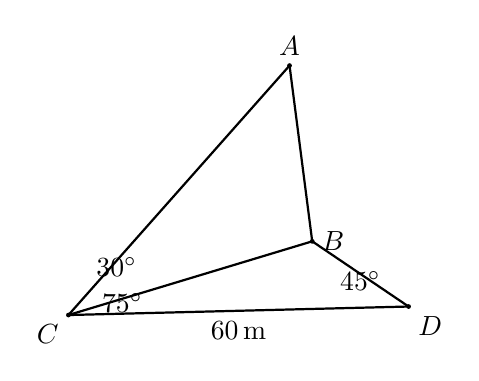
\begin{tikzpicture}[scale=0.72,>=stealth]
  \coordinate (C) at (0,0);
  \coordinate (D) at (6,0.15);
  \coordinate (B) at (4.3,1.3);
  \coordinate (A) at (3.9,4.4);
  \draw[thick] (C)--(A);
  \draw[thick] (C)--(B);
  \draw[thick] (C)--(D);
  \draw[thick] (D)--(B);
  \draw[thick] (A)--(B);
  \fill (A) circle (1.2pt) node[above] {$A$};
  \fill (B) circle (1.2pt) node[right] {$B$};
  \fill (C) circle (1.2pt) node[below left] {$C$};
  \fill (D) circle (1.2pt) node[below right] {$D$};
  \node at (0.85,0.85) {$30^\circ$};
  \node at (0.95,0.22) {$75^\circ$};
  \node at (5.15,0.6) {$45^\circ$};
  \node[below] at (3,0.05) {$60\,\mathrm{m}$};
\end{tikzpicture}
\end{center}
\nopagebreak[4]
\end{question}
\begin{question}
\gkti{7}

（1） 画出抛物线 $y=x^2+2$ 的图象，并写出它的顶点坐标、对称轴的方程和极值；

（2） 如果上述抛物线的顶点作为新的坐标原点 $O_1$，把它的对称轴作为新的纵轴 $O_1Y_1$，求这抛物线在新的直角坐标系 $X_1O_1Y_1$ 中的方程，并写出它的准线方程和焦点坐标。

\end{question}
\begin{question}
\gkti{8}某工厂四年来的产量，第一年到第三年的产量是按等差数列增长的，三年的总产量共 $1500$ 吨；第二年到第四年的产量是按等比数列增长的，这三年的产量共 $1820$ 吨。求每年的产量各是多少吨？

\Needspace{0.4\textheight}
\end{question}
\begin{question}
\gkti{9}三角形 $ABC$ 中，$AE$ 和 $BD$ 相交于 $G$（如图），已知 $AD:DC=3:1$，$BG=GD$，求：$\dfrac{AG}{GE}$。
\nopagebreak[4]
\begin{center}% 1977 年江苏镇江地区初试卷第 9 题：三角形 ABC 中，D 在 AC 上（AD:DC=3:1），
% E 在 BC 上，AE 与 BD 相交于 G（BG=GD），按源卷第 3 页布局
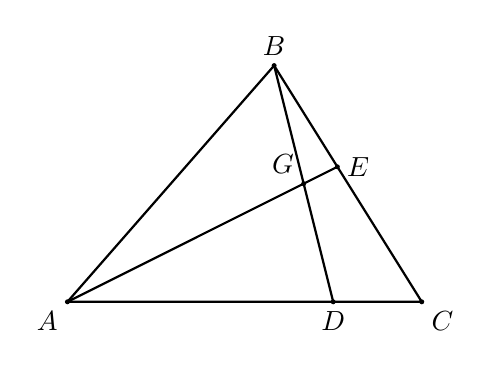
\begin{tikzpicture}[scale=0.75]
  \coordinate (A) at (0,0);
  \coordinate (C) at (6,0);
  \coordinate (B) at (3.5,4);
  \coordinate (D) at (4.5,0);
  \coordinate (E) at (4.571,2.286);
  \coordinate (G) at (4,2);
  \draw[thick] (A)--(B)--(C)--cycle;
  \draw[thick] (A)--(E);
  \draw[thick] (B)--(D);
  \fill (A) circle (1.2pt) node[below left] {$A$};
  \fill (B) circle (1.2pt) node[above] {$B$};
  \fill (C) circle (1.2pt) node[below right] {$C$};
  \fill (D) circle (1.2pt) node[below] {$D$};
  \fill (E) circle (1.2pt) node[right] {$E$};
  \fill (G) circle (1.2pt) node[above left] {$G$};
\end{tikzpicture}
\end{center}
\nopagebreak[4]

\end{question}